\chapter{Alternujúce stroje}

V predchádzajúcich kapitolách sme si ukázali viaceré paralelné
modely. I keď šlo \mbox{o rôzne} pohľady na paralelizmus, všetky
mali jedno spoločné: pozerali sa na vec z ``gramatikového''
pohľadu, teda vo všetkých prípadoch sme mali jednu, prípadne
viacero gramatík, ktoré čosi generovali. Teraz si ukážeme jednu
automatovú charakterizáciu a porovnáme ju so sekvenčnými triedami.
Pre čitateľa, ktorý sa s pojmom alternovania ešte nestretol,
povedzme nasledovných pár viet. Modely alternujúcich strojov sa
uvažujú pre všetky známe zariadenia, my si ich popíšeme na
najvšeobecnejšom prípade, teda na Turingových strojoch, pre
čitateľa iste nebude problémom analogicky si zadefinovať
alternujúce konečné automaty, alternujúce zásobníkové automaty,
prípadne alternujúce lineárne ohraničené automaty. O niektorých
týchto zariadeniach si v závere kapitoly ukážeme pár zaujímavých
vecí, napr. ako alternovanie ovplyvní, resp. neovplyvní ich
generatívnu silu a podobne. Zariadenie (alternujúci stroj) má tzv.
existenčné a tzv. univerzálne stavy, ktoré môže ľubovoľne
kombinovať, a ktoré si ďalej bližšie popíšeme. Alternujúci
Turingov stroj sa v existenčných stavoch správa rovnako, ako už
známy nedeterministický model Turingovho stroja. Odlišné je
správanie sa v univerzálnych stavoch. Zariadenie sa akoby rozdelí
na $n$ nových strojov (kde $n$ je počet konfigurácií
dosiahnuteľných na 1 krok z jeho momentálnej konfigurácie), ktoré
dostanú novú pamäť (rovnakú ako pôvodný stroj) a ďalej nezávisle
od seba pracujú, táto operácia sa nazýva FORK a čitateľovi môže
byť trošku v reálnejšej podobe známa z niektorých operačných
systémov (UNIX), kde jeden proces vytvára nové a prideľuje im
pamäť.

\section{Definície a označenia}

\begin{definicia}
Alternujúci Turingov stroj (ATS) je 6-tica
$A=(K,\Sigma,\Gamma,\delta,q_0,F)$, kde $K$ je konečná množina
stavov rozdelená na dve disjunktné časti $K=K_1\cup K_2$, $K_1$ je
množina exis\-tenčných stavov, $K_2$ je množina univerzálnych
stavov, $\Sigma$ je abeceda vstupných symbolov, $\Gamma$ je
pracovná (pásková) abeceda, $q_0$ je počiatočný stav a $F$ je
množina akceptačných stavov, $\delta$ je prechodová funkcia
\[
\delta:K\times\Gamma\ra 2^{K\times\Gamma\times\{-1,0,1\}}
\]
\end{definicia}

\begin{definicia}
Konfiguráciu ATS $A$ definujeme rovnako ako pre nedeterministické
Turingove stroje (NTS), bližšie napr. \cite{Hopc}
\end{definicia}

\begin{definicia}
Krok výpočtu ATS $A$ je relácia $\vdash$ na konfiguráciách
definovaná rovnako ako pre NTS
\end{definicia}

Čitateľ si možno spomenie na pojem stromu konfigurácií, definovaný
pre nedeterministický Turingov stroj, ktorý prehľadne
reprezentoval jeho výpočet na konkrétnom slove\footnote{bol napr.
dobrou pomôckou pri dôkaze ekvivalencie deteministických a
nedeterministických Turingových strojov}. Podobný strom definujeme
aj pre alternujúce stroje. Okrem toho, že nám tento pojem pomôže
pri definovaní výpočtu ATS, mal mi výraznou mierou prispieť k
pochopeniu alternovania samotného.

\begin{definicia}
Úplný strom konfigurácií pre ATS $A$ a vstupné slovo $w$ je strom,
ktorého vrcholy sú označené konfiguráciami taký, že:
\begin{enumerate}
\item koreň je počiatočná konfigurácia na slove $w$
\item každý vrchol má za priamych nasledovníkov práve toľko
vrcholov, koľko konfigurácii je v relácii $\vdash$ s konfiguráciou
označujúcou daný vrchol
\item tieto vrcholy sú označené týmito konfiguráciami
\end{enumerate}
\end{definicia}

\begin{poznamka}
Úplný strom konfigurácií nemusí byť konečný
\end{poznamka}

\begin{definicia}
Výpočet ATS $A$ (na slove $w$) je podstrom úplného stromu
konfigurácií na slove $w$ taký, že:
\begin{enumerate}
\item obsahuje koreň
\item s každým univerzálnym vrcholom $(q\in K_2)$ obsahuje
všetkých jeho priamych nasledovníkov
\item s každým existenčným vrcholom obsahuje práve jedného jeho
priameho nasledovníka, ak existuje
\end{enumerate}
\end{definicia}

\begin{definicia}
Akceptujúci výpočet ATS $A$ na slove $w$ je taký výpočet na $w$,
ktorý je konečný a každá listová konfigurácia je akceptačná
\end{definicia}

\begin{definicia}
Jazyk akceptovaný ATS $A$ je
\[
L(A)=\{w\in\Sigma^*\mm \mbox{existuje akceptačný výpočet}\ A\
\mbox{na}\ w\}
\]
\end{definicia}

\begin{priklad}\label{dvojhlavy}
Ukážeme si, ako alternovanie pomôže dvojhlavým konečným
automatom\footnote{budeme uvažovať zariadenie s možnosťou pohybu
hlavy iba jedným smerom} v ge\-ne\-ra\-tív\-nej sile. Zoberme si
jazyk $L=\{ww\mm w\in\{a,b\}^*\}$. Dalo by sa ukázať, že ho nie je
možné akceptovať dvojhlavým konečným automatom, no zostrojíme preň
alternujúci dvojhlavý konečný automat, ktorý bude pracovať
nasledovne:
\begin{enumerate}
\item dostane na vstup slovo, nedeterministicky uhádne jeho
polovicu
\item nastane FORK, automat alternuje v univerzálnom stave
\begin{itemize}
\item 1. proces overuje, či vstup je tvaru $ww$ tak, že hlavy sa
synchrónne pohybujú po vstupe, v jednom kroku každá číta symbol,
ak obe prečítajú to isté a keď sa jedna z nich dostane na koniec
vstupu, dôjde k akceptovaniu
\item 2. proces overuje, či automat uhádol polovicu správne tak,
že prvá hlava sa hýbe o jedno políčko vpravo, zatiaľ čo za ten
istý čas sa druhá hlava hýbe o dve políčka vpravo, k akceptovaniu
dôjde, ak obe hlavy dočítajú naraz vstupné slovo
\end{itemize}
\end{enumerate}
Výpočet automatu možno vidieť na (obr.\ref{apreww})
\end{priklad}

\begin{figure}[!ht]
\centering
\includegraphics{img/apreww}
\caption{Úplný strom konfigurácií automatu pre jazyk $L=\{ww\mm
w\in\{a,b\}^*\}$} z príkladu \ref{dvojhlavy} \label{apreww}
\end{figure}

\begin{veta}
$\mathcal{L}_{ATS}=\mathcal{L}_{RE}$
\end{veta}

\begin{dokaz}
Povieme si pár slov o oboch inklúziách:
\begin{description}
\item{$\subseteq$:} vyplýva z Turingovej tézy, keby sme mali
zkonštruovať TS, ktorý by simuloval ATS, tak by sme zrejme
prechádzali strom konfigurácii ATS do šírky, pamätali si niečo o
výpočte a charaktere stavov a podobne
\item{$\supseteq$:} na NTS sa možno pozerať aj ako na špeciálny
prípad ATS, keď akoby všetky stavy NTS boli existenčné
\end{description}
\end{dokaz}

\section{Miery zložitosti}

Pre ATS si zadefinujeme dve miery, ktoré sú analógiou mier
$NSPACE,NTIME$ definovaných pre NTS:

\begin{itemize}
\item $ASPACE=$ najväčší počet použitých políčok na páske v
niektorej konfigurácii akceptačného výpočtu
\item $ATIME=$ hĺbka akceptačného výpočtu v strome
konfigurácií
\end{itemize}

V niektorých simuláciách budeme pracovať s triedou jazykov
$ATIME(f(n))$, $\log n<f(n)<n$. Klasický model ATS by sme tu
nemohli použiť, lebo na prečítanie vstupu dĺžky $n$ potrebujeme
aspoň $n$ krokov. V takýchto prípadoch sa používa model ATS s
rýchlym prístupom na vstup. Môžeme si ho reprezentovať nasledovne:
nad páskou má binárny vyhľadávací strom, každý list je práve jedno
políčko, strom má výšku $\log n$, máme register dĺžky $\log n$,
keď do neho binárne zapíšeme číslo $k$, tak za čas $\log n$ sa
dostaneme ku $k$-temu vstupnému políčku (obr.\ref{rychly}).

\begin{figure}[!ht]
\centering
\includegraphics{img/rychly}
\caption{Model ATS s rýchlym prístupom na vstup} \label{rychly}
\end{figure}

\section{Alternujúce vs. sekvenčné triedy zložitosti}

Keďže vo väčšine simulácií budeme požadovať predpoklad páskovej
konštruovateľnosti nejakej funkcie, bude dobré, keď si tento pojem
zadefinujeme.

\begin{definicia}
Funkcia $f(n)$ sa nazýva páskovo konštruovateľná, ak existuje
deterministický Turingov stroj (DTS) $T$, ktorý je $f(n)$ páskovo
ohraničený a vyznačí na páske $f(n)$ políčok
\end{definicia}

Ukazuje sa, že takmer všetky funkcie, ktoré si možno reálne
predstaviť, sú páskovo konštruovateľné, problémy pri
konštruovateľnosti však nastávajú, keď sa pozrieme na triedu
funkcií menších ako $\log n$, teda $O(\log n)$. Keby sme chceli
nahliadnuť medzi nekonštruovateľné funkcie, dobrým prostriedkom na
ich zostrojovanie by bola metóda diagonalizácie.

\smallskip
V tejto chvíli sme už pripravení na ukázanie základného výsledku o
alternujúcich Turingových strojoch.

\begin{veta}
\label{alter_veta_nspaceatime} $NSPACE(S(n))\subseteq ATIME(S^2(n))$ pre
$S(n)\geq\log n$
\end{veta}

\begin{dokaz}
Ak $S(n)\geq n$, nie je problém v lineárnom čase prečítať vstup,
ak by však bolo $S(n)<n$, na prečítanie vstupu našim ATS $A'$ by
sme potrebovali aspoň lineárny čas a celá simulácia by ztroskotala
už na začiatku. Preto použijeme model ATS s rýchlym prístupom na
vstup, v logaritmickom čase $O(\log n)$ sa vieme dostať na
ľubovoľné políčko vstupnej pásky, využívame tu ideu paralelnej
práce procesov, nie každý proces musí vidieť celý vstup, aby
akceptoval, resp. každému procesu bude k práci stačiť malý úsek
vstupu. K danému NTS $A$ pracujúcemu v priestore $S(n)$ zostrojíme
ATS $A'$ pracujúci v čase $S^2(n)$ taký, že $L(A)=L(A')$.

\smallskip
Akceptujúci výpočet $A$ na slove $w$ dĺžky $n$ má (zmysluplne)
dĺžku najviac $c^{S(n)}$ pre vhodné\footnote{ako už neraz,
$c^{S(n)}$ je počet rôznych konfigurácií $A$ na slove dĺžky $n$,
keď máme k dispozícii priestor $S(n)$} $c$. Položme $m=c^{S(n)}$,
$\forall i\med k_i$ je konfigurácia $A$, akceptujúci výpočet má
tvar:
\[
k_1\vdash k_2\vdash\dots\vdash k_m
\]
pričom $k_1$ je počiatočná konfigurácia, $k_m$ je akceptačná
konfigurácia (ak je náhodou akceptujúci výpočet kratší,
dodefinujeme $\delta$-funkciu v akceptačnom stave tak, aby sa nič
nedialo, ale aby sme mohli ``naťahovať'' výpočet).

\smallskip
ATS $A'$ bude pracovať nasledovne:
\begin{enumerate}
\item výpočet začne v $k_1$
\item uhádne akceptačnú konfiguráciu $k_m$
\item overí, či sa z $k_1$ do $k_m$ dá dostať na $m$ krokov
nasledovne:
\begin{enumerate}
\item uhádne $k_{\frac{m}{2}}$
\item overí, či sa z $k_1$ dá dostať do $k_{\frac{m}{2}}$ na $\frac{m}{2}$
krokov
\item overí, či sa z $k_{\frac{m}{2}}$ dá dostať do $k_m$ na $\frac{m}{2}$
krokov
\end{enumerate}
\end{enumerate}
Body b) a c) tretieho kroku sú vlastne rekurzívne volania kroku 3
s parametrami $k_1,k_{\frac{m}{2}},\frac{m}{2}$, resp.
$k_{\frac{m}{2}},k_m,\frac{m}{2}$. ATS $A'$ sa do rekurzie bude
vnárať\footnote{každé rekurzívne volanie si môžme reprezentovať z
hľadiska alternovania tak, že $A'$ vytvorí nový proces, ktorý ako
parametre dostane $k_i,k_j,r$ a za úlohu má overiť, či sa z $k_i$
dá dostať do $k_j$ na $r$ krokov (obr.\ref{ats_time})} dovtedy,
kým sa nedostane na úroveň, kedy bude overovať, či sa dá z $k_i$
dostať do $k_{i+1}$ na jeden krok $\forall i=1,\dots,m-1$
(obr.\ref{aspace1}). Táto úroveň je z hľadiska rekurzie
elementárna, na nej stačí overiť, či v $\delta$-funkcii NTS $A$
existoval taký prechod, ktorý umožnil prepísanie konfigurácie
$k_i$ na $k_{i+1}$ (teda simulujeme jeden krok pôvodného NTS $A$).
Je nutné si uvedomiť, že rekurzia sa vykonáva paralelne.

\begin{figure}[!ht]
\centering
\includegraphics{img/aspace1}
\caption{Overovanie náveznosti konfigurácií v ATS $A'$}
\label{aspace1}
\end{figure}

Pozrime sa na proces hádania konfigurácií a overovania
dosiahnuteľnosti konfigurácie $k_j$ z konfigurácie $k_i$ na $m$
krokov podrobnejšie, z hľadiska alternovania a rozdelenia množiny
stavov ATS $A'$ na existenčné a univerzálne. Na začiatku výpočtu
je $A'$ v stave $q_0$ a na vstupe má slovo $w$, teda $k_1=q_0 w$,
tento stav je existenčný. Teraz $A'$ prejde do stavu $q_H$ a háda
$k_m$, pod $q_0 w$ v strome konfigurácií visí ``veľmi košatý''
strom (označme ho $N$), je na (obr.\ref{strom_n}), výšky $S(n)$,
ktorý ako všetky svoje vrcholy, vrátane listov, obsahuje všetky
možné konfigurácie NTS $A$ v priestore $S(n)$. Kvôli jednoduchosti
si ho môžeme popísať nasledovne\footnote{konfigurácia ako ju
popisujeme, neobsahuje stav, ani pozíciu hlavy, čitateľ si tieto
veci iste rád domyslí sám} (na čitateľa nechávame domyslenie
ukončenia generovania):
\[
\delta(q_H,1)=\{(q_H,a,1),(q_H,b,1)\}
\]

\begin{figure}[!ht]
\centering
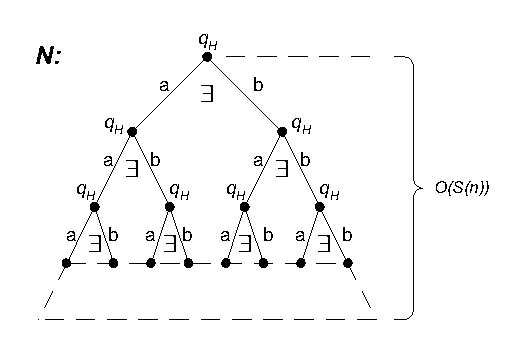
\includegraphics{img/strom_n}
\caption{Hádanie konfigurácie dĺžky $S(n)$ ATS $A'$}
\label{strom_n}
\end{figure}

Keď má $A'$ uhádnutú akceptačnú konfiguráciu $k_m$, overí, či sa z
$k_1$ do $k_m$ dá dostať na $m$ krokov. To spraví tak, že uhádne
$k_{\frac{m}{2}}$ rovnako, ako hádal $k_m$ (teda pod každým
vrcholom stromu $N$ visí nový strom (opäť rovnaký ako $N$, má
odlišné stavy, všetky sú existenčné), v ktorom $A'$ háda
$k_\frac{m}{2}$). Keď ju uhádne, overuje, či sa z $k_1$ dá dostať
do $k_{\frac{m}{2}}$ na $\frac{m}{2}$ krokov a či sa z
$k_{\frac{m}{2}}$ dá dostať do $k_m$ na $\frac{m}{2}$ krokov tak,
že v univerzálnom stave spraví FORK dvoch nových
procesov\footnote{to je práve jedno rekurzívne volanie}, ktoré
pracujú paralelne a každý overuje polovicu toho, čo mal overiť
materský proces, atď.

\begin{figure}[!ht]
\centering
\includegraphics{img/ats_time}
\caption{Schématické vytváranie nových procesov ATS $A'$}
\label{ats_time}
\end{figure}

Z konštrukcie by malo byť zrejmé (nebudeme to dokazovať), že
$L(A)=L(A')$. Poďme sa teraz pozrieť na časovú zložitosť ATS $A'$,
ktorý sme práve zkonštruovali: máme $O(S(n))$ rekurzívnych volaní
a v každom hádame strednú konfiguráciu, resp. na začiatku musíme
uhádnuť akceptačnú konfiguráciu $k_m$. Hádanie ľubovoľnej
konfigurácie $k_i$ trvá čas $O(S(n))$, čo je presne výška stromu
$N$, lebo ju treba zapamätať na páske. Celkový počet krokov (alebo
inak výška akceptačných vetiev úplného stromu konfigurácií) $A'$
je $O(S^2(n))$ a teda $L(A')\in ATIME(S^2(n))$
\end{dokaz}

\begin{poznamka}
V predchádzajúcej vete sme použili ``paralelnú verziu''
konštrukcie, ktorá bola (v sevkvenčnej podobe) použitá pri dôkaze
vety $NSPACE(S(n))\subseteq DSPACE(S^2(n))$ (Savitch)
\end{poznamka}

Pri väčšine známych konštrukcií, keď máme dané zariadenie
(Turingov stroj) a požadujeme k nemu zostrojiť zariadenie
ekvivalentné, ale rýchlejšie, urýchlenie ide na úkor použitého
priestoru, resp. analogicky keď požadujeme zmenšenie použitého
priestoru, ide to na úkor času. Ako naznačila konštrukcia z vety
\ref{alter_veta_nspaceatime}, pri alternujúcich strojoch je situácia trochu
iná. Pozornému čitateľovi iste neunikol fakt, že priestorové
ohraničenie zostrojeného ATS zostalo nezmenené.

\smallskip
V niektorých konštrukciách bude kôli jednoduchosti vhodné uvažovať
binárne vetvenie úplného stromu konfigurácií ATS, teda fakt, že
ľubovoľný prechod $\delta$-funkcie má najviac dva prvky. Ukážeme
si preto nasledovné dve tvrdenia o normálnych tvaroch pre ATS.

\begin{lema}\label{binarny_nt}
K ľubovoľnému ATS $A$ pracujúcemu v čase $T(n)$ s ľubovoľnou
veľkosťou vetvenia\footnote{veľkosťou vetvenia rozumieme maximálny
počet konfigurácii dosiahnuteľný z ľubovoľnej konfigurácie na
jeden krok} v úplnom strome konfigurácii existuje ATS $A'$
pracujúci v čase $T(n)$, ktorého úplný strom konfigurácii je
binárny a $L(A)=L(A')$
\end{lema}

\begin{dokaz}
Iba neformálne naznačíme spôsob konštrukcie $A'$: nech je vetvenie
vo vrchole $v$ úplného stromu konfigurácií $A$ stupňa $n$. Binárne
vetvenie vytvoríme tak, že v ľavej vetve vychádzajúcej z vrchola
$v$ bude jeho najľavejší nasledovník a v pravej všetci ostatní
nasledovníci tak, že priamy nasledovník $v$ bude $v'$ a jeho
nasledovníci budú zvyšnými nasledovníkmi $v$. Konfiguráciu v tomto
vrchole dostaneme tak, že v konfigurácii vo $v$ zmeníme stav na
nový, ktorý ešte nepatrí do množiny stavov $A$, vetvenie vrchola
$v'$ bude stupňa $n-1$, teda o 1 menšieho ako vetvenie $v$. Na
vrchol $v'$ aplikujeme algoritmus rekurzívne a v rekurzii skončíme
až vtedy, keď bude vrchol stupňa $\leq2$. Na čitateľa nechávame
premysieť, ako algoritmus aplikovať na celý strom
konfigurácií\footnote{pomôcka: $\delta$-funkcia $A$ má iba konečne
veľa prvkov a vetvenie v úplnom strome konfigurácií je iba
grafické znázornenie $\delta$-funkcie, resp. výpočtu}. Dodajme
ešte, že ak vrchol $v$ bol existenčný, tak aj všetky vrcholy,
ktoré pri vytváraní binárneho vetvenia vzniknú, budú existenčné,
podobne ak $v$ bol univerzálny, tak všetky vzniknuté vrcholy budú
univerzálne. Uvedomme si, že hĺbka akceptačného výpočtu v úplnom
strome konfigurácií $A'$ bude iba konštantným násobkom hĺbky
úplného stromu konfigurácií $A$, teda $A'$ pracuje v čase $T(n)$ a
akceptuje rovnaký jazyk ako $A$
\end{dokaz}

\begin{lema}\label{binarny_nt2}
K ľubovoľnému ATS $A$ pracujúcemu v priestore $S(n)$ s ľubovoľnou
veľkosťou vetvenia v úplnom strome konfigurácii existuje ATS $A'$
pracujúci v priestore $S(n)$, ktorého úplný strom konfigurácii je
binárny a $L(A)=L(A')$
\end{lema}

\begin{dokaz}
V konštrukcii z lemy \ref{binarny_nt} sme nikde nemenili priestor,
ktorý využíval $A$ pri práci, a teda tvrdenie je jej priamym
dôsledkom
\end{dokaz}

Nasledujúce tvrdenie hovorí, ako efektívne z hľadiska
priestorového ohraničenia vieme simulovať alternujúce Turingove
stroje pracujúce v čase $T(n)$ na deterministických Turingových
strojoch.

\begin{veta}
\label{atimedspace} $ATIME(T(n))\subseteq DSPACE(T(n))$ pre
$T(n)\geq\log n, T(n)$ je páskovo konštruovateľná
\end{veta}

\begin{dokaz}
V celom dôkaze budeme pod pojmom strom konfigurácii rozumieť
podstrom úplného stromu konfigurácii, ktorý dostaneme tak, že v
úplnom strome konfigurácii ``odrežeme'' všetky vetvy v hĺbke
$T(n)$.

\smallskip
K danému ATS $A$ pracujúcemu v čase $T(n)$ zostrojíme DTS $A'$
pracujúci v priestore $T(n)$. Podľa lemy \ref{binarny_nt} môžeme
kvôli jednoduchosti predpokladať, že úplný strom konfigurácii $A$
je binárny. $A'$ musí overiť, či sa v strome konfigurácií $A$
nachádza podstrom akceptujúceho výpočtu.

\smallskip
$A'$ bude prehľadávať strom konfigurácií $A$ algoritmom PREORDER
do hĺbky a priradzovať vrcholom hodnoty $0,1$ nasledovne:
\begin{itemize}
\item vrcholu sa môže priradiť hodnota iba vtedy, ak sú už
priradené hodnoty všetkým jeho nasledovníkom v strome konfigurácii
alebo ak je to list\footnote{listom sa v tomto prípade myslí aj
taký vrchol, ktorý síce nie je listovým v úplnom strome
konfigurácii $A$, ale stáva sa listovým vrcholom v strome
konfigurácii $A$}
\item listom priradzujeme hodnoty podľa toho, či sú akceptujúcimi,
alebo neakceptujúcimi konfiguráciami, akceptujúcim priradíme
hodnotu 1, neakceptujúcim hodnotu 0
\item ak je vrchol existenčný (a nie je to list)
a aspoň jeden z jeho nasledovníkov v strome konfigurácii má
hodnotu $1$, tak sa mu priradí hodnota $1$, inak sa mu priradí $0$
\item ak je vrchol univerzálny (a nie je to list), tak sa mu priradí
hodnota 1 práve vtedy, keď obaja jeho nasledovníci v strome
konfigurácií majú hodnotu 1, inak sa mu priradí 0
\end{itemize}
$A'$ akceptuje svoj vstup práve vtedy, keď bude koreňu priradená
hodnota 1. Keby sme chceli dosiahnuť dobrý pomer čas/priestor, asi
by sme postupovali tak, že by sme si pamätali informáciu o celom
``lúči'' konfigurácii, teda všetky konfigurácie, ktorými sme od
koreňa prechádzali až k listom, resp. ku vrcholom v hĺbke $T(n)$,
aby sme nestrácali čas pri vracaní sa v strome smerom nahor.
Dosiahli by sme však priestorové ohraničenie $T^2(n)$ (pretože by
sme si museli pamätať až $T(n)$ konfigurácií, každú dĺžky $T(n)$),
čo v našom prípade nie je žiadúce, preto budeme musieť použiť
trochu rafinovanejšiu konštrukciu, vzhľadom na to, že nám nezáleží
na čase. Nebudeme si pamätať celý ``lúč'' konfigurácii, ale iba
momentálnu konfiguráciu a navigáciu k nej v strome konfigurácii.
Navigácia bude dĺžky najviac $T(n)$ a bude to postupnosť z
$\{0,1\}^*$, kde 0 znamená pohyb v strome vľavo smerom dole a 1
znamená pohyb vpravo smerom dole. Keď sa budeme v strome musieť
vracať smerom hore, tak si predchodcu konfigurácie, v ktorej práve
sme, podľa tejto navigácie vypočítame, na páske $A'$
(obr.\ref{paska}) si budeme potrebovať pamätať navigáciu,
momentálnu konfiguráciu a pár pomocných konfigurácii, teda máme
priestorové ohraničenie $T(n)$ pre $A'$
\end{dokaz}

\begin{figure}[!ht]
\centering
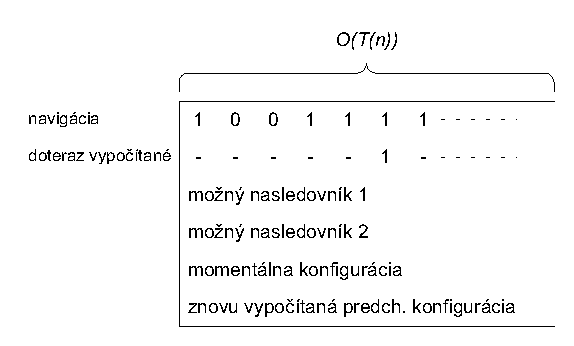
\includegraphics{img/paska}
\caption{Páska DTS $A'$ (druhá stopa by sa dala pamätať aj v
stave)} \label{paska}
\end{figure}

\begin{definicia}
Polynomiálne triedy zložitosti definujeme nasledovne:
\begin{itemize}
\item $NSPACE(Poly)\overset{def}=\underset{{k\geq1}}{\bigcup}NSPACE(n^k)$
\item $DSPACE(Poly)\overset{def}=\underset{{k\geq1}}{\bigcup}DSPACE(n^k)$
\item $ATIME(Poly)\overset{def}=\underset{{k\geq1}}{\bigcup}ATIME(n^k)$
\end{itemize}
\end{definicia}

\begin{dosledok} \label{alter_dosl_nspacepolyatimepoly}
$NSPACE(Poly)=DSPACE(Poly)=ATIME(Poly)$
\end{dosledok}

\begin{dokaz}
Tvrdenie vyplíva zo Savitchovej vety, vety \ref{alter_veta_nspaceatime} a
vety \ref{atimedspace}
\end{dokaz}

\begin{veta}
$ASPACE(S(n))\subseteq\underset{{c>0}}{\bigcup}DTIME(c^{S(n)})$
pre $S(n)\geq\log n$
\end{veta}

\begin{dokaz}
Ukážeme si, že keď máme k ATS $A$ pracujúcemu v priestore $S(n)$
zostrojiť DTS $A'$ pracujúci v exponenciálnom čase $c^{S(n)}$ pre
nejaké nezáporné $c$, tak nám na simuláciu postačí aj veľmi hrubá
sila, akou je bezosporu vygenerovanie všetkých možných
konfigurácii $A$ na páske a práca na týchto konfiguráciách. Opäť
budeme bez újmy na všeobecnosti predpokladať, že úplný strom
konfigurácií $A$ je binárny.

\smallskip
$A'$ bude pracovať nasledovne:
\begin{itemize}
\item na pásku zapíše všetkých $|\Gamma_A|^{S(n)}.S(n).|K_A|<r^{S(n)}$
konfigurácii $A$ v lexikografickom usporiadaní, za každou
konfiguráciou si nechá priestor (jedno políčko), ktorý ďalej
využije\footnote{priestor si na páske vyznačíme napr. $\#?\#$,
pričom $\#$ slúži ako oddeľovač konfigurácii, nie je prvkom
páskovej abecedy $\Gamma$, rovnako ani $?$, ktorý hovorí, že o
tomto políčku zatiaľ nič nevieme}, na to potrebuje čas
$S(n).r^{S(n)}$
\item do vyznačeného priestoru bude každej konfigurácii
priraďovať hodnoty $0,1,?$ prechodom stromu konfigurácii $A$ tak,
že v každom prechode priradí hodnoty $0,1$ rodičom tých detí,
ktoré už sú vyhodnotené a hodnotu $?$ rodičom nevyhodnotených detí
(podľa (obr.\ref{exponent})), akceptuje, ak bude počiatočnej
konfigurácii priradená hodnota $1$, časová zložitosť bude
nasledovná:
\begin{enumerate}
\item $r^{S(n)}$-krát prejde pásku a ``spracuje'' každú konfiguráciu
\item ``spracovať'' konfiguráciu znamená zistiť hodnoty jej
nasledovníkov a ak sa dá, tak jej priradiť hodnotu 0,1, toto je
časovo ohraničené $\approx r^{S(n)}.S(n)$
\end{enumerate}
\end{itemize}
Keď si celú prácu $A'$ zosumarizujeme, dostávame časovú zložitosť
približne $c^{S(n)}$ pre nejaké $c$ (stačí zvoliť napr.
$c=r^{10}$) a sme hotoví
\end{dokaz}

\begin{figure}[!ht]
\centering
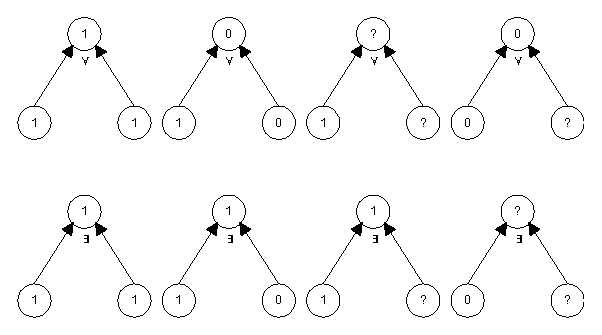
\includegraphics{img/exponent}
\caption{Priraďovanie hodnôt rodičom v strome konfigurácii ATS
$A$} \label{exponent}
\end{figure}

\begin{veta}
\label{dtime_aspace}
$DTIME(T(n))\subseteq ASPACE(\log T(n))$ pre $T(n)\geq n$
\end{veta}

\begin{dokaz}
Nech $A_1$ je $k$-páskový DTS pracujúci v čase $T(n)$. K nemu
existuje jednopáskový DTS $A=(K_A,\Sigma,\Gamma,\delta,q_0,F_A)$
pracujúci v čase $T^2(n)$ taký, že $L(A_1)=L(A)$. K nemu
zkonštruujeme ATS $A'$ pracujúci v priestore $\log T(n)$ taký, že
$L(A)=L(A')$. Najskôr si zapíšme konfigurácie $A$ pod seba podľa
(obr.\ref{dts_ats}) tak, že v prvom riadku bude počiatočná
konfigurácia $q_0w$ a keď označíme $<qw_k>_{l}$ konfiguráciu v
$k$-tom riadku pre nejaký stav $q\in K_A$ a pozíciu stavu (hlavy)
v tejto konfigurácii $l$, tak platí
$<qw_k>_{l}\vdash<pw_{k+1}>_{m}$, pričom $m\in\{l-1,l,l+1\}$. Ak
$w\in L(A)$, tak máme v tabuľke zapísanú postupnosť konfigurácií
akceptujúceho výpočtu (vzhľadom na to, že $A$ je deterministický),
teda existuje $i$ také, že pre $<q_Fw_i>_j$ je $q_F\in F_A$.

\begin{figure}[!ht]
\centering
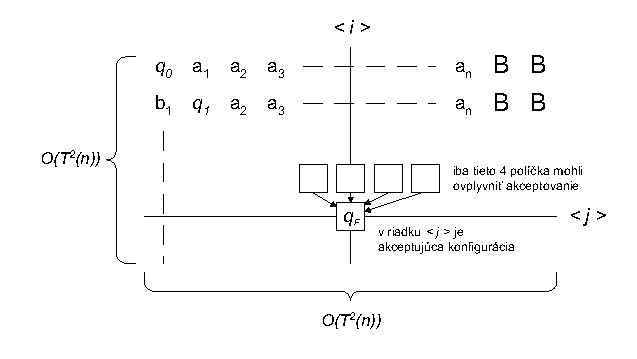
\includegraphics{img/dts_ats}
\caption{Tabuľka konfigurácií jednopáskového DTS $A$}
\label{dts_ats}
\end{figure}

$A'$ bude pracovať nasledovne:
\begin{itemize}
\item uhádne pozíciu $<$riadok, stĺpec$>$ akceptačného stavu $q_F$
v akceptujúcej kon\-fi\-gu\-rá\-cii tvaru \mbox{$<q_Fw_i>_j$},
teda háda $<i,j>$, toto zaberie $\log T^2(n)$ políčok (môžeme
zvoliť napr. binárnu reprezentáciu čísel $i,j$), to je $2.\log
T(n)\approx\log T(n)$ políčok
\item uhádne, ktorý akceptujúci stav sa na pozícii $<i,j>$
nachádza
\item overí, či dobre hádal pozíciu $<i,j>$ a akceptačný stav
nasledovne:
\begin{enumerate}
\item uhádne (zmysluplne\footnote{podľa $\delta$-funkcie $A$})
obsahy políčok
\mbox{$<i-1,j-1>,<i-1,j>,<i-1,j+1>$},\\\mbox{$<i-1,j+2>$}, pretože
týmito obsahmi je obsah $<i,j>$ jednoznačne určený
\item v univerzálnom vetvení overí, či hádal správne (každá
vetva overí jedno políčko)
\end{enumerate}
Takto sa bude $A'$ vracať v tabuľke až do prvého riadku (zrejme si
bude dekrementovať $i$ a pracovať s $j$ podľa pohybu hlavy $A$),
keď bude na pozícii $<1,1>$ a bude v počiatočnom stave, tak
akceptuje
\end{itemize}
Pri prechode tabuľkou konfigurácií smerom zdola nahor sa nám
nemôže stať, že by sme našli viac ako jednu cestu vedúcu k
akceptovaniu, pretože $A$ je deterministický a teda akceptačný
výpočet pre dané slovo je vždy jednoznačný, ak sme v niektorej
vetve niečo zle uhádli, výpočet sa určite zablokuje.

\smallskip
Keď sa máme baviť o priestorovej zložitosti $A'$, jediná vec,
ktorá ju ovplyvňuje, je dĺžka $i$, resp. $j$, pretože okrem týchto
dvoch čísel si pamätáme iba konštantne veľa informácii (dokonca
veľmi málo). Ale o dĺžke sme si už povedali, že je $\log T(n)$,
takže sme hotoví
\end{dokaz}

\begin{dosledok}
$ASPACE(S(n))=\underset{{c>0}}{\bigcup}DTIME(c^{S(n)})$ pre
$S(n)\geq n$
\end{dosledok}

\section{Alternujúce konečné automaty ($AFSA$)}

Čitateľ sa iste stretol s viacerými modifikáciami pôvodného modelu
deterministických konečných automatov. Nedeterminizmus im
nepomohol, rovnako ako nepomohlo napr. pridanie možnosti
obojsmerného pohybu po vstupnej páske. Mohlo by sa zdať, že taká
sila, akou je alternovanie, by mohlo pomôcť týmto zariadeniam
vyjsť z triedy $\mathcal{R}$ a akceptovať aj nejaké nie regulárne
jazyky. Ako však hovorí nasledujúca veta, opak je pravdou. Faktom
totiž zostáva, že keď procesom v jednotlivých vetvách neumožníme
komunikáciu, resp. synchronizáciu, tak sa sila zariadenia
nezväčší.

\begin{veta}
$\mathcal{L}_{AFSA}=\mathcal{R}$
\end{veta}

\begin{dokaz}
\label{afsa_r} Inklúzia zprava doľava je triviálna a preto ju
nebudeme ukazovať. Na dôkaz opačnej inklúzie zostrojíme k AFSA $A$
ekvivalentný nedeterministický konečný automat (NKA) $A'$ taký, že
\mbox{$L(A)=L(A')$}. Najskôr podobnou konštrukciou ako pre NKA
zostrojíme k $A$ ekvivalentný ATS $A_1$ (teda platí $L(A)=L(A_1)$)
taký, že v $A_1$ neexistujú $\varepsilon$-prechody (konštrukcii sa
nebudeme bližšie venovať, čitateľ ju nájde napr. v \cite{Hopc}).
Zavedieme pár označení, ktoré sa nám neskôr budú hodiť:
\begin{itemize}
\item $all(q,a)=\{$množina všetkých stavov dosiahnuteľných v $A_1$ na
jeden krok zo stavu $q$ pri čítaní vstupného symbolu $a\}$
\item $ex_i(q,a)=p$, pričom $p\in\delta'(q,a)$ a keď máme prvky
$\delta'(q,a)$ očíslované, resp. usporiadané, tak $\delta'(q,a)=p$
je $i$-ty v poradí
\end{itemize}
Teraz k bez-$\varepsilon$ ATS $A_1=(K,\Sigma,\delta,q_0,F)$
zostrojíme NKA $A'=(K',\Sigma',\delta',q'_0,F')$ nasledovne:
\begin{itemize}
\item Vezmime si úplný strom konfigurácii $A_1$ a pozrime sa naň
po úrovniach. Keďže v $A_1$ nie sú $\varepsilon$-prechody, tak na
$n$-tej úrovni je zo vstupu prečítaných práve $n$-symbolov
\item $K'$ bude nová množina stavov, pričom jej prvky budú podmnožiny
množiny stavov $K$, teda počet stavov $|K'|=2^{|K|}$, formálne
\[
[q_{i_1},\dots,q_{i_k}]\in K'\overset{def}{\Longleftrightarrow}
q_{i_1},\dots,q_{i_k}\in K
\]
\item $\Sigma'=\Sigma$, teda vstupná abeceda sa nemení
\item $\delta'$ definujeme nasledovne:
\begin{itemize}
\item ak $q$ je univerzálny a $\delta(q,a)=\{q_{i_1},\dots,q_{i_k}\}$, tak
$\delta'([q],a)=\{[q_{i_1},\dots,q_{i_k}]\}$
\item ak $q$ je existečný a $\delta(q,a)=\{q_{i_1},\dots,q_{i_k}\}$, tak
$\delta'([q],a)=\{[q_{i_1}],\dots,[q_{i_k}]\}$
\item rekurzívne definujeme
$\delta'([q_{i_1},\dots,q_{i_j},q_{i_{j+1}}, \dots,q_{i_k}],a)$
ako\\ $\{[all(q_{i_1},a),
\dots,all(q_{i_j},a),ex_1(q_{i_{j+1}},a)],
\dots,[all(q_{i_1},a),\dots,all(q_{i_j},a),ex_n(q_{i_k})]\}$\\
pri\-čom $q_{i_1},\dots,q_{i_j}$ sú univerzálne stavy a
$q_{i_{j+1}},\dots,q_{i_k}$ sú existenčné stavy a platí
$|\delta'(q_{i_k})|=n$
\end{itemize}
V stavoch $A'$ udržujeme informácie o všetkých vetvách úplného
stromu konfigurácií $A_1$, je dobré si uvedomiť, že ak už máme
množinu stavov $[p,q]$, a napr. $\delta'([p],a)=[r]$ a súčasne
$\delta'([q],a)=[r]$, tak si túto informáciu nemusíme pamätať
druhý krát, ako stav si budeme pamätať iba $[r]$
\item prirodzene definujeme $q'_0=[q_0]$
\item $F'=\{[q_{i_1},\dots,q_{i_k}]\mm q_{i_1},\dots q_{i_k}\in F\}$
\end{itemize}
Nemalo by byť až také ťažké pochopiť, že $L(A_1)=L(A')$, a teda
platí aj $L(A)=L(A')$
\end{dokaz}

V niektorých konštrukciách je potrebné a zmysluplné požadovať, aby
zostrojený konečný automat k alternujúcemu konečnému automatu bol
deterministický. Potom jeho stavy budú opäť množiny stavov AFSA,
keď tieto budú univerzálne, no keď prídu do hry exis\-ten\-čné
stavy, tak sa stavy rozpadnú na množiny, akceptačné stavy potom
budú také, ktorých aspoň jedna zložka je akceptačná v už
definovanm nedeterministickom zmysle. Stavov môže byť až
$2^{2^{|K|}}$, čo nie je zanedbateľné číslo.

\begin{priklad}
Ku AFSA $A=(K,\Sigma,\delta,q_0,F)$, ktorého úplný strom
konfigurácií na $w=aba$ je na (obr.\ref{afsa_aka}), pričom
$\{q_0,\dots,q_4,p_1,p_2,r_1,\dots,r_4\}\subseteq K$,
$\Sigma=\{a,b\}$, $\{r_1,r_2,r_3\}\subseteq F$ a $\delta$ je
zrejmá z obrázku\footnote{definovali sme iba časť AFSA $A$
potrebnú pre výpočet na $w$}, zostrojíme NKA
$A'=(K',\Sigma',\delta',q'_0,F')$ (jeho časť) podľa konštrukcie z
vety \ref{afsa_r} nasledovne:
\begin{enumerate}
\item
$\{[q_0],[p_1,p_2],[q_1,q_3],[q_1,q_4],
[q_2,q_3],[q_2,q_4],[r_1,r_2,r_3],[r_2,r_3,r_4]\}\subset K'$
\item $\Sigma'=\Sigma$
\item $q'_0=[q_0]$
\item $[r_1,r_2,r_3]\subseteq F'$
\item $\delta'$ definujeme schématicky nasledovne:
\begin{displaymath}
[q_0]\overset{a}{\rightsquigarrow}[p_1,p_2]\overset{b}{\rightsquigarrow}
\left\{
\begin{array}{l}
{[q_1,q_3]}\overset{a}{\rightsquigarrow}
\left\{
\begin{array}{l}
{[r_1,r_2,r_3]}\\
{[r_2,r_3,r_4]}
\end{array}
\right.
\\
{[q_1,q_4]}\overset{a}{\rightsquigarrow}
\left\{
\begin{array}{l}
{[r_1,q_4]}\\
{[r_4,q_4]}
\end{array}
\right.
\\
{[q_2,q_3]}\overset{a}{\rightsquigarrow}
{[q_2,r_2,r_3]}
\\
{[q_2,q_4]}\overset{a}{\rightsquigarrow}{[q_2,q_4]}
\end{array}
\right.
\end{displaymath}
\end{enumerate}
Potom zrejme výpočet
\[
[q_0]aba\vdash_{A'}[p_1,p_2]ba\vdash_{A'}[q_1,q_3]a
\vdash_{A'}[r_1,r_2,r_3]
\]
je akceptujúcim výpočtom NTS $A'$ na $w$.
\end{priklad}

\begin{figure}[!ht]
\centering
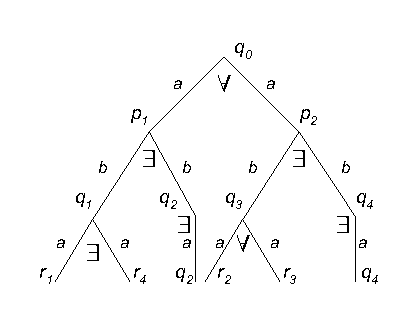
\includegraphics{img/afsa_aka}
\caption{Úplný strom konfigurácií AFSA $A$ na slove $w=aba$}
\label{afsa_aka}
\end{figure}

\section{Alternujúce zásobníkové automaty ($APDA$)}

Ako sme ukázali, konečným automatom alternovanie v generatívnej
sile vôbec nepomohlo. Lepšia je situácia v oblasti bezkontextových
jazykov, ktoré rozpoznávajú zásobníkové automaty (PDA). Tu
alternovanie zvýši možnosť rozpoznávania jazykov až na úroveň, o
ktorej hovorí nasledujúce tvrdenie

\begin{veta}\label{apda}
$\underset{c}{\bigcup} DTIME(c^n)\subseteq\mathcal{L}_{APDA}$
\end{veta}

\begin{dokaz}
Tvrdenie nebudeme dokazovať priamo, využijeme tvrdenie vety
\ref{dtime_aspace}, podľa ktorého platí $\underset{c}{\bigcup}
DTIME(c^n)\subseteq ASPACE(n)$. My ukážeme, že platí
$ASPACE(n)\subseteq\mathcal{L}_{APDA}$, potom bude z tranzitívnosti
relácie $\subseteq$ platiť aj
$\underset{c}{\bigcup}DTIME(c^n)\subseteq\mathcal{L}_{APDA}$.

\smallskip
Na dôkaz $ASPACE(n)\subseteq\mathcal{L}_{APDA}$ potrebujeme k
ATS $A$, ktorý pre vstup dĺžky $n$ používa $n$ políčok na
pracovnej páske, zostrojiť APDA $A'$ taký, že
$L(A)=L(A')$. Bez újmy na všeobecnosti budeme predpokladať, že
úplný strom konfigurácií $A$ je binárny\footnote{čitateľ si
iste vie predstaviť podobnú konštrukciu ako v leme
\ref{binarny_nt2} pre APDA}.

\smallskip
$A'$ bude pracovať nasledovne\footnote{idea je nasledovná: v
zásobníku bude simulovať výpočet ATS $A$ tak, že do neho bude
postupne pridávať konfigurácie $A$ a overovať ich náväznosť
vzhľadom na $\vdash$, keď pridá do zásobníka akceptačnú
konfiguráciu, ktorá bude nadväzovať na predchádzajúce, akceptuje}:
\begin{itemize}
\item najskôr v existenčnom vetvení uhádne počiatočnú
konfiguráciu (bude hádať $n+1$ symbolov, háda aj stav) $q_0w$,
pričom $w=a_1\dots a_n$, v obrátenom poradí, teda zásobník bude
mať po $n+1$ krokoch tvar ako na (obr.\ref{zasobnik1}a)
\item v univerzálnom vetvení v jednej vetve overí, či konfiguráciu
hádal správne, v druhej vetve háda nasledovníkov konfigurácie
$q_0w$ vo vetvení, ktorého typ zodpovedá vetveniu v úplnom strome
konfigurácií $A$, každej konfigurácii priradí aj vetvu, v ktorej
sa nachádzala v úplnom strome konfigurácií $A$ (teda L,R),
konfigurácie ďalej overí a háda ďaľšie, až kým neakceptuje, resp.
neodmietne (REJECT) vstup
\item do overenia, či konfigurácie na seba nadväzujú, spadá:
\begin{itemize}
\item overiť, či sme hádali správnu vetvu (prvky $\delta_A$
si usporiadame L,R)
\item $A'$ musí po jednotlivých symboloch prejsť konfigurácie a
testovať ich na rovnosť (obr.\ref{zasobnik1}b), resp. možnosť
prechodu v $\delta_A$, univerzálne sa rozvetví: v jednej vetve
overí, či sa 1. symbol zhoduje s ($n+k$)-tym symbolom\footnote{$k$
je konštanta, jej určenie prenechávame na čitateľa}, resp.či
existuje v $\delta_A$ prechod taký, aby sa symboly na seba mohli
prepísať, tak, že zo zásobníka zmaže $n+k$ symbolov (je dôležité
uvedomiť si, že do tejto chvíle sme v tejto vetve vstup nečítali,
tu ho používame na počítanie $n$, zrejme bude dobre vždy si v
stave pamätať 4 symboly z vrchu pôvodného obsahu zásobníka pred
vymazávaním), v ďaľšej overí, či 2. až ($n+1$)-vý symbol z prvej
konfigurácie sedí podľa $\delta_A$ s 2. až ($n+1$)-vým symbolom
druhej konfigurácie podobne ako pre 1. symbol
\end{itemize}
\end{itemize}
Čitateľovi odporúčame podrobnejšie rozpracovať overovanie
konfigurácii, najmä overenie, či sa konfigurácia nachádzala v
ľavej, alebo pravej vetve vzhľadom na svojho predka, v úplnom
strome konfigurácií ATS $A$. Na pochopenie, že $L(A)=L(A')$ by
však úroveň detailu v našej konštrukcii mala byť dostačujúca
\end{dokaz}

\begin{figure}[!ht]
\centering
\includegraphics{img/zasobnik1}
\caption{Zásobník APDA $A'$ a) po uhádnutí $q_0w$ b) pri overovaní
náväznosti konfigurácií} \label{zasobnik1}
\end{figure}

\begin{poznamka}
Platí aj obrátená inklúzia, jej dôkaz však presahuje rozsah tohto
textu, navyše na ukážku, že alternovanie zásobníkovým automatom
pomáha v generatívnej sile, stačí veta \ref{apda}
\end{poznamka}

\section{Synchronizované alternujúce stroje}

Ukážeme si jednu modifikáciu pôvodného modelu alternujúcich strojov,
keď umožníme jed\-no\-du\-chú komunikáciu medzi paralelnými procesmi.
Zavedieme nové delenie stavov alternujúceho
stroja, nezávisle od delenia na existenčné a univerzálne stavy,
na:
\begin{itemize}
\item obyčajné
\item synchronizačné - dvojica $(q,S)\ra($stav,symbol$)$
\end{itemize}
Keď proces prejde do synchronizačného stavu, čaká, kým všetky
ostatné prejdu do synchronizačného stavu. Keď majú všetky rovnaký
symbol v druhej komponente synchronizačného stavu, pokračujú,inak
sa zariadenie zablokuje

\begin{priklad}
Ukážeme si, že keď umožníme synchronizáciu konečným automatom, tak
sa nám ich podarí posunúť z triedy regulárnych jazykov. Na
(obr.\ref{anbnc}) je znázornený synchronizovaný konečný automat,
ktorý akceptuje bezkontextový jazyk $L=\{a^nb^nc\mm n\geq1\}$
\end{priklad}

\begin{figure}[!ht]
\centering
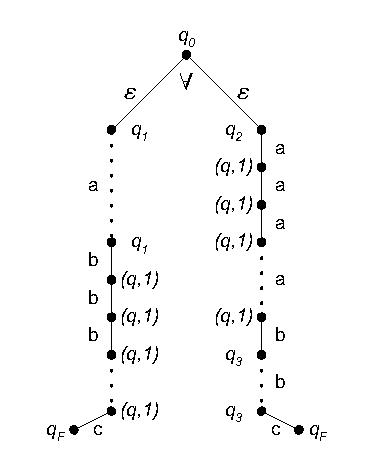
\includegraphics{img/anbnc}
\caption{Synchronizovaný konečný automat pre jazyk $L=\{a^nb^nc\mm
n\geq1\}$} \label{anbnc}
\end{figure}

\begin{poznamka}
Dá sa ukázať tvrdenie, ktoré hovorí o tom, že trieda jazykov
rozpoznávaných synchronizovanými konečnými automatmi je presne
$\mathcal{L}_{CS}$
\end{poznamka}
